\begin{center}
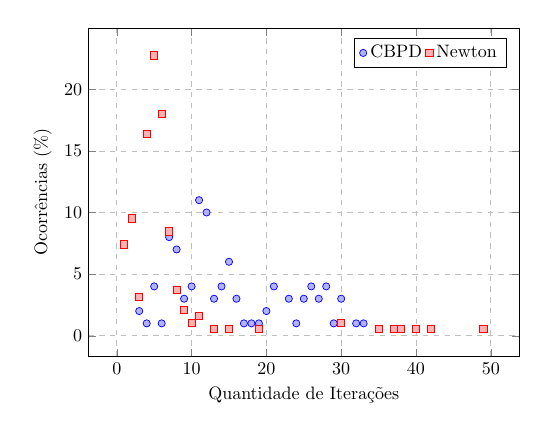
\begin{tikzpicture}[scale = 0.65]
  \begin{axis}[
    width=10cm,
    height=8cm,
    xlabel={Quantidade de Iterações},
    ylabel={Ocorrências (\%)},
    legend style={at={(0.5,-0.2)}, anchor=north, legend columns=-1},
    grid=major,
    grid style=dashed,
    legend pos=north east
  ]

    % First set of data
    \addplot[
      only marks,
      mark=*,
      color=blue,
      fill=blue!30,
    ] coordinates {
        (12, 10.00)
        (11, 11.00)
        (5, 4.00)
        (13, 3.00)
        (14, 4.00)
        (15, 6.00)
        (9, 3.00)
        (7, 8.00)
        (23, 3.00)
        (16, 3.00)
        (8, 7.00)
        (30, 3.00)
        (32, 1.00)
        (19, 1.00)
        (33, 1.00)
        (21, 4.00)
        (20, 2.00)
        (25, 3.00)
        (26, 4.00)
        (28, 4.00)
        (27, 3.00)
        (29, 1.00)
        (10, 4.00)
        (18, 1.00)
        (17, 1.00)
        (24, 1.00)
        (6, 1.00)
        (4, 1.00)
        (3, 2.00)
      };

    % Second set of data
    \addplot[
      only marks,
      mark=square*,
      color=red,
      fill=red!30,
    ] coordinates {
        (6, 17.99)
        (5, 22.75)
        (4, 16.40)
        (2, 9.52)
        (7, 8.47)
        (3, 3.17)
        (9, 2.12)
        (8, 3.70)
        (10, 1.06)
        (11, 1.59)
        (35, 0.53)
        (38, 0.53)
        (40, 0.53)
        (30, 1.06)
        (13, 0.53)
        (1, 7.41)
        (15, 0.53)
        (49, 0.53)
        (42, 0.53)
        (37, 0.53)
        (19, 0.53)
    };
    \legend{CBPD, Newton}

  \end{axis}
\end{tikzpicture}
\end{center}
